\documentclass{beamer}
 
\usepackage[utf8]{inputenc}
\usepackage{amsmath}
\usefonttheme{serif} % default family is serif
 
 
%Information to be included in the title page:
\title{Approximation preserving reductions}
\author{Cesare Lingua}
\institute{Università degli Studi di Torino}
\date{} 
\beamertemplatenavigationsymbolsempty
\setbeamertemplate{footline}{%
    \raisebox{5pt}{\makebox[\paperwidth]{\hfill\makebox[10pt]{\scriptsize\insertframenumber}}}} 
\begin{document}
 
\frame{\titlepage}

 
 
\begin{frame}
\frametitle{La riduzione:}
    \begin{block}{Idea:}
        Trasformare un problema $A$ in un altro problema $B$ in modo tale che risolvendo $B$ si possa ricavare anche una soluzione per $A$.

    \end{block}
    \begin{block}{Vantaggi:}
        \begin{itemize}
            \item trasferire tecniche di risoluzione da un problema all'altro;
            \item studiare la complessità dei problemi, cioè, la classe di complessità a cui appartengono.
        \end{itemize}
    \end{block}

\end{frame}

\begin{frame}
\frametitle{Approximation preserving reductions:}
    \begin{itemize}
        \item $f$ mappa un istanza $x$ del problema $A$ in un istanza $f(x)$ del problema $B$
        \item $g$ mappa una soluzione ammissibile $y$ di $B$ in una soluzione ammissibile $g(x)$ di $A$  con la proprietà che $g(y)$ è una soluzione \textit{approssimata} del problema $A$ 
    \end{itemize}

    \begin{center}
    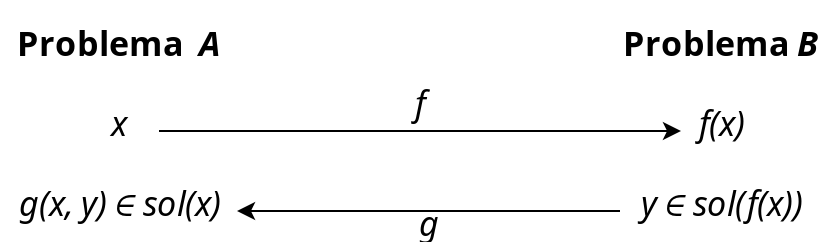
\includegraphics[width=\textwidth]{../images/schema.png}
    \end{center}
    
\end{frame}

\begin{frame}
    \frametitle{Vantaggi dell'approximation preserving reductions:}
        \begin{itemize}
         \item Permette di trasferire le tecniche di \textit{approssimazione} da un problema $B$ ad un problema $A$;
         \item Studiare limiti di approssimazione dei problemi, cioè, se sappiamo che il problema $B$ non può essere approssimato oltre un certo limite, lo stesso vale per $A$;
         \item Differenziare le classi di complessità.
        
        \end{itemize}        
\end{frame}

\begin{frame}
\frametitle{Problema di Ottimizzazione NP:}
    \begin{block}{\underline{Definizione} (NPO)}
        Un \textit{problema di Ottimizzazione} $\Pi \in$ \textbf{NP}, abbreviato \textbf{NPO},  è una quadrupla ($I$, $Sol$, $\textbf{m}$, $goal$), tale che:
        \begin{itemize}
            \item $I$ è l'insieme delle istanze, riconoscibili in tempo polinomiale, di $\Pi$; 
            \item dato $x\in I$, $Sol(x)$ denota l'insieme delle \textit{soluzioni ammissibili} di $x$; per ogni $y \in Sol(x)$, $|y|$ (la dimensione di $y$) è polinomiale in $|x|$ (la dimensione di $x$); dato una qualsiasi istanza $x$ e qualsiasi soluzione $y$ si può decidere in tempo polinomiale se $y \in Sol(x)$;
            \item data $x \in I$ e $y \in Sol(x)$, $\textbf{m}(x, y)$ denota il valore di $y$ è può essere caclolato in tempo polinomiale;
            \item $goal\in\{max, min\}$ denota il \textit{tipo} di problema di ottimizzazione.
        \end{itemize}
    \end{block}

\end{frame}

\begin{frame}
    \frametitle{Algoritmo di approssimazione:}
    
    Dato $\Pi = (I, Sol, m, goal)$, problema \textbf{NPO}, una soluzione ottima di un istanza $x$ di $\Pi$ è indicata con $y^{*}(x)$ e il suo valore $\textbf{m}(x,y^{*}(x))$ con $opt(x)$.
    \vskip 15pt
    \begin{block}{\underline{Definizione} (Algoritmo di approssimazione)}
        Dato $\Pi = (I, Sol, m, goal)$, problema \textbf{NPO}, un \textit{algorimo di approssimazione} $A$ è un algoritmo che data un instanza $x$ di $\Pi$ restituisce una soluzione ammissibile $y \in Sol(x)$. Se $A$  esegue in tempo polinomiale rispetto a $|x|$, si dice che $A$ è un \textit{algoritmo di approssimazione polinomiale} di $\Pi$.
    \end{block}
    \vskip 20pt
    La qualità della soluzione di un algoritmo di approssimazione $A$ è misurata con il \textit{rapporto di approssimazione} $\rho_A(x)$
    $$\rho_A(x) = \max \Bigg \{\frac{\textbf{m}(x, A(x))}{opt(x)}, \frac{opt(x)}{\textbf{m}(x, A(x))} \Bigg\} $$ 
%     tra il valore della soluzione approssimata, $m(x, A(x))$, e il valore ottimo della soluzione $opt(x)$.
\end{frame}

\begin{frame}
    \frametitle{Classi dei problemi di ottimizzazione:}
    \begin{block}{\underline{Definizione} (APX)}
        Un problema \textbf{NPO} $\Pi$ appartiene alla classe \textbf{APX} se esiste un \textit{\underline{algoritmo} di approssimazione polinomiale} $A$ e un valore $r \in \mathbb{Q}$, tale che, data un'istanza $x$ di $\Pi$, vale, $\rho_A(x) \le r$. In questo caso $A$ è detto algoritmo di $r-$approssimazione.
    \end{block}
    \vskip 20pt
    \begin{block}{\underline{Definizione} (PTAS)}
        Un problema \textbf{NPO} $\Pi$ appartiene alla classe \textbf{PTAS} se esiste uno \textit{\underline{schema} di approssimazione polinomiale} $A_r$, tale che, per ogni $r \in \mathbb{Q}, r \neq 1$ e una qualsiasi istanza $x$ di $\Pi$, vale,  $\rho_{A_r}(x) \leq r$.
 
    \end{block}
\end{frame}

\begin{frame}
    \frametitle{Classi dei problemi di ottimizzazione:}
    \begin{block}{\underline{Definizione} (FPTAS)}
        Un problema \textbf{NPO} $\Pi$ appartiene alla classe \textbf{FPTAS} se esiste uno \textit{\underline{schema} di approssimazione polinomiale} $A_r$, tale che, dato un qualsiasi valore $r \in \mathbb{Q}, r \neq 1$, e una qualsiasi istanza $x$ di $\Pi$, vale, $ \rho_{A_r}(x) \leq r$. Inoltre, esiste un polinomio $q$ che limita il tempo di esecuzione di $A_r(x)$ a $q(x,1/(r-1))$.
    \end{block}
    \vskip 50 pt
    Sotto l'ipotesi di $\textbf{P} \neq \textbf{NP}$ le classi sopra descritta formano la segenete catena di inclusioni strette: $\textbf{FPTAS} \subset \textbf{PTAS} \subset \textbf{APX} \subset \textbf{NPO}$
\end{frame}

\begin{frame}
    \frametitle{Riduzione base: R-riduzione}
    \begin{block}{\underline{Definizione} (R-riduzione)}
        Siano $\Pi_1$ e $\Pi_2$ due problemi \textbf{NPO}. Allora diciamo che $\Pi_1$ è R-riducibile a $\Pi_2$ e si scrive $\Pi_1 \leq_R \Pi_2$, se esistono due funzioni polinomiali $f, g$ che soddisfano le seguenti proprietà:
        \begin{itemize}
         \item $f: I_{\Pi_1}\rightarrow I_{\Pi_2} $, tale che $\forall x_1 \in I_{\Pi_1}, f(x_1)\in I_{\Pi_2}$;  in altre parole, data un istanza $x_1$ in $\Pi_1$, $f$ permette di costruire un istanza $x_2 = f(x_1)$ in $\Pi_2$;
         \item $g:I_{\Pi_1} \times Sol_{\Pi_2} \rightarrow Sol_{\Pi_1}$, tale che, $\forall (x_1, y_2)\in(I_{\Pi_1} \times Sol_{\Pi_2}(f(x_1))), g(x_1, y_2)\in Sol_{\Pi_1}(x_1)$ ; in altre parole, partendo dalla soluzione $y_2$ dell'istanza $x_2$, $g$ determina la soluzione $y_1 = g(x_1, y_2)$ dell'istanza iniziale $x_1$. 
        \end{itemize}
    \end{block}
\end{frame}

% \begin{frame}
%     \frametitle{Chiusura}
%     \begin{block}{\underline{Definizione} (Chiusura)}
%         Sia \textbf{C} una classe di problemi \textbf{NPO} e $X$ un tipo di riduzione. Allora, la chiusura $\boldsymbol{\overline{C}^{X}}$ di \textbf{C} per $X$ e definita come: $\boldsymbol{\overline{C}^{X}} = \{\Pi \in \boldsymbol{NPO}: \exists \Pi' \in \boldsymbol{C}, \Pi \le_X \Pi'\}$
%     \end{block}
% 
% \end{frame}

\begin{frame}
    \frametitle{Riduzione Lineare: L-riduzione}
    \begin{block}{\underline{Definizione} (L-riduzione)}
        Siano $\Pi$ e $\Pi'$ due problemi in \textbf{NPO}. Allora, diciamo che $\Pi$ è L-riducibile a $\Pi'$, e si scrive $\Pi \leq_L \Pi'$, se esistono due funzioni $f$ e $g$ e due costanti $\alpha > 0$ e $\beta > 0$ tali che $\forall x \in I_{\Pi}$ e $\forall y' \in Sol_{\Pi'}(f(x))$:
        \begin{itemize}
         \item $opt_{\Pi'}(f(x)) \leq \alpha\ opt_{\Pi}(x)$;
         \item $|\textbf{m}_{\Pi}(x, g(y'))- opt_{\Pi}(x)| \leq \beta\ |\textbf{m}_{\Pi'}(f(x), y') - opt_{\Pi'}(f(x))|$.
        \end{itemize}
    \end{block}
    \begin{block}{Proprietà:}
        Dati due problemi $\Pi$ e $\Pi'$, se $\Pi \leq_L \Pi'$ e 
        $\Pi' \in \textbf{PTAS}$,allora, $\Pi \in \textbf{PTAS}$. In altre parole, la L-riduzione preserva l'appartenenza a \textbf{PTAS}.
    \end{block}

    
\end{frame}

\begin{frame}
    \frametitle{Esempio L-riduzione}
    
    \begin{block}{MAX k-SAT}
        Dato un istanza $\varphi$ composta da $m$ clausole in CNF, ciascuna con $k$ letterali $l^{k}_i$, con $i=1,...,m$, trovare un assegnamento di valori di verità che massimizzi il numero di clausole soddisfatte.

    \end{block}
    \vskip 40pt
    \begin{block}{Teorema}
        $$MAX \text{ 3-SAT} \le_L MAX \text{ 2-SAT}$$
    \end{block}

    


\end{frame}

\begin{frame}
    \frametitle{Esempio L-riduzione}
    \begin{block}{Dimostrazione}
        Data un istanza $\varphi$ di MAX 3-SAT con $m$ clausole $C_i$ con $i = 1,...,m$, siano $l_i^1 \vee l_i^2 \vee l_i^3$ le tre variabili dell'$i$-esima clausola, e $l_i^1, l_i^2 $ e $ l_i^3$ possono rappresentare o una variabile oppure la sua negazione.\\
        A ciascuna delle $m$ clausole associamo le seguenti dieci nuove clausole, composte al più da due letterali: $l_i^1, l_i^2, l_i^3, l_i^4, \bar l_i^1 \vee \bar l_i^2, \bar l_i^1 \vee \bar l_i^3, \bar l_i^2 \vee \bar l_i^3, l_i^1 \vee \bar l_i^4, l_i^2 \vee \bar l_i^4, l_i^3 \vee \bar l_i^4$, dove $l_i^4$ è una nuova variabile.
    \end{block}

\end{frame}

\begin{frame}
    \frametitle{Esempio L-riduzione}
    Sia $C_i'$ la congiunzione delle dieci clausole derivanti da $C_i$. Usando la formula $\varphi' = f(\varphi)$ generiamo la congiunzione di tutte le clausole $C_i'$ con $i = 1,...,m$. Quindi $ \varphi' = f(\varphi) = \bigwedge\limits_{i = 1}^m C_i'$ dove $\varphi'$ è un istanza di MAX 2-SAT.\\
    Si osserva che:
    \begin{itemize}
        \item ogniqualvolta $C_i$ è \textit{vera}, allora si può trovare un valore di verità per $l_i^4$ in modo tale che esattamente \textbf{sette} clausole in $C_i'$ siano \textit{vere}:
            \begin{itemize}
                \item[-] se $l_i^1, l_i^2,l_i^3$ sono tutte \textit{veri}, pongo $l_i^4 = vero$;
                \item[-] se esattemente un letterale $l_i^1, l_i^2,l_i^3$ è \textit{vero}, pongo $l_i^4 = falso$;
                \item[-] altrimeni, $l_i^4$ può essere indifferentemente $vero$ o $falso$.
                \end{itemize}
        \item se $C_i$ è \textit{falsa}, quindi $l_i^1, l_i^2,l_i^3$ sono tutti \textit{falsi}, allora ponendo $l_i^4$ a \textit{falso} esattamente {sei} clausole $C_i'$ sono \textit{vere}.
    \end{itemize}
    

    
\end{frame}

\begin{frame}
    \frametitle{Esempio L-riduzione}
    Quindi avremo che:\\
    $$opt(\varphi')= 6m + opt(\varphi)$$
    Inoltre, grazie al seguente lemma:
    \begin{block}{Lemma 1}
        Data una formula in CNF, almeno la metà delle clausole può sempre essere soddisfatta.
    \end{block}
    Avremo che, in quanto $\frac{1}{2}m \leq opt(\varphi)\Rightarrow m \leq 2opt(\varphi)$:
    $$ opt(\varphi') \leq opt(\varphi)+12opt(\varphi) = 13opt(\varphi) $$
    

\end{frame}

\begin{frame}
    \frametitle{Esempio L-riduzione}
    Per ogni assegnamento \textit{vero} $\tau'$ per le variabili di $\varphi'$, la restrizione $g(\varphi, \tau') = \tau$ , ottenuta eliminando le $l_i^4$, è tale che:
    \begin{equation}
        \begin{split}
            opt(\varphi)-\textbf{m}(\varphi, \tau) & = opt(\varphi')-6m-\textbf{m}(\varphi, \tau) \\
            & \leq opt(\varphi')-6m -\textbf{m}(\varphi', \tau')+6m\\
            &= opt(\varphi')-\textbf{m}(\varphi', \tau')
        \end{split}
    \end{equation}
\end{frame}

\begin{frame}
    \frametitle{Esempio L-riduzione}
    Mettendo insieme i risultati ottenuti avremo che:
        \begin{itemize}
     \item $ opt(\varphi') \leq  13opt(\varphi) $
     \item $ opt(\varphi)-\textbf{m}(\varphi, \tau) \leq opt(\varphi')-\textbf{m}(\varphi', \tau') $ 
    \end{itemize}
    Ponendo $\alpha = 13$ e $\beta = 1$ abbiamo si verificano le due disequanzioni necessarie per avere una L-riduzione
\end{frame}


\begin{frame}
    \frametitle{S-riduzione}
    L-riduzione non garantise un importante caratteristica, cioè che riducendo un problema $\Pi_1$ a un problema $\Pi_2$, la soluzione $y_1$ del problema di partenza $\Pi_1$ ottenuta grazie \textit{mapping} di $g$ sia almeno "buona" come la soluzione $y_2$ ottenuta da $\Pi_2$.\\
    La \textit{strict reduction} (S-riduzione) garantisce questa propietà
    \begin{block}{\underline{Definizione} (S-riduzione)}
     Siano $\Pi_1$ e $\Pi_2$ due problemi \textbf{NPO}. Allora, diciamo che $\Pi_1 \leq_S \Pi_2$ se esistono due funzioni polinomiali calcolabili $f$, $g$ che soddisfano la seguente proprietà:
     $$\forall x\in I_{\Pi_1}, \forall y \in Sol_{\Pi_2}(f(x)), \rho_ {\Pi_2}(f(x), y) \geq \rho_{\Pi_1}(x, g(x, y)) $$
    \end{block}


\end{frame}

\begin{frame}
    \frametitle{S-riduzione}
    \begin{block}{Proprietà 1}
        Dati due problemi $\Pi_1$ e $\Pi_2$, se $\Pi_1 \leq_S \Pi_2$ e $\Pi_2 \in \textbf{APX}$, allora $\Pi_1 \in \textbf{APX}$ 
    \end{block}
    \begin{block}{Proprietà 2}
        Dati due problemi $\Pi_1$ e $\Pi_2$, se $\Pi_1 \leq_S \Pi_2$ e $\Pi_2 \in \textbf{PTAS}$, allora $\Pi_1 \in \textbf{PTAS}$ 
    \end{block}


\end{frame}

\begin{frame}
    \frametitle{Esempio S-riduzione}
    \begin{block}{Teorema}
        \begin{center}
            \scalebox{0.8}{
            MIN WEIGHTED VERTEX COVER $\leq_S$ MIN VERTEX COVER
        }
        \end{center}
    \end{block}
    \begin{block}{Dimostrazione}
        Consideriamo un istanza $(G(V, E), \vec{w})$ di MIN WEIGHTED VERTEX COVER  in cui i pesi dei \underline{vertici} sono limitati da un polinomio $p(n)$   
        e mostriamo come trasformarla in un instanza $G'(V', E')$ di MIN VERTEX COVER. Procediamo con i seguenti passaggi:
        \begin{enumerate}
         \item per ogni vertice $v_i\in V$ con peso $w_i$ costruiamo un insieme indipendente $W_i$ con $w_i$ nodi;
         \item per ogni arco $(v_i, v_j) \in E $ costruiamo un grafo bipartito completo tra i vertici dei due insiemi indipendenti $W_i$ e $W_j$ in $G'$
        \end{enumerate}

    \end{block}
\end{frame}

\begin{frame}
    \frametitle{Esempio S-riduzione}
%     $$
        \begin{center}
            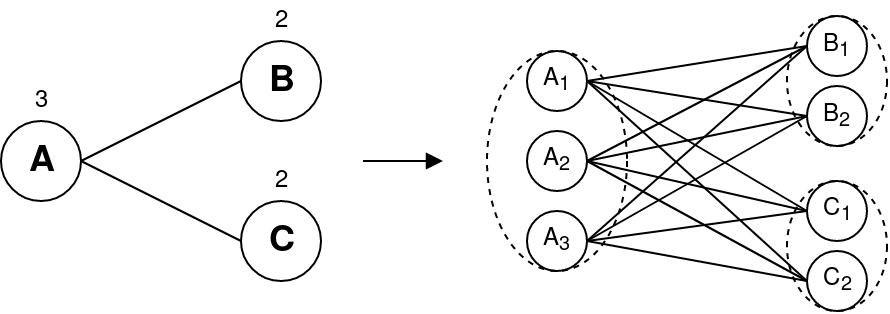
\includegraphics[width=\textwidth]{../images/GtoG'.png}
        \end{center}
        Questa operazione è polinomiale poiche il grafo risultante $G'$ ha $\sum_{i=1}^{n}w_i \leq np(n)$ vertici.
        
\end{frame}

\begin{frame}
    %A vertex cover of an undirected graph is a subset of its vertices such that for every edge (u, v) of the graph, either ‘u’ or ‘v’ is in vertex cover. Although the name is Vertex Cover, the set covers all edges of the given graph. Given an undirected graph, the vertex cover problem is to find minimum size vertex cover%
    \frametitle{Esempio S-riduzione}
    Consideriamo adesso una copertura minima $C'$ di $G'$ e dimostriamo che $C'$ è composto da $l$ inisiemi indipendenti $W_i$ i cui nodi sono tutti inclusi o esclusi.\\
    Assumiamo per assurdo il contratio:
    \begin{itemize}
     \item consideriamo un insime $W_k$ solo parzialmente incluso in $C'$;
     \item consideriamo anche gli insiemi indipendenti $W_p$, connsessi ai vertici di $W_k$, che possono essere interamente o parzialmente inclusi in $C'$.
    \end{itemize}
\end{frame}

\begin{frame}
    \frametitle{Esempio S-riduzione}
    Si possono verificare due casi:
    \begin{enumerate}
     \item tutti gli insiemi $W_p$ hanno i loro vertici inclusi in $C'$; in questo caso $C'$ non sarebbe più una copertura minimale;
     \item tra gli inemi $W_p$ esiste almeno un insieme $W_q$ i cui vertici $W_q'$ sono solo parzialmente inclusi in $C'$.
    \end{enumerate}
    Nel secondo caso poichè il sottografo di $G'$ prodotto da $W_k \cup W_q$ è bipartito completo, gli archi che connettono i vertici di $W_p \backslash W_p' $ con quelli di $W_q\backslash W_q'$ non sono inclusi nella copertura di $C'$, contraddicendo l'assunzione precedente.\\
    Allora possiamo definire una funzione $g$ nel seguente modo:\\
    Se $C'$ è una copertura di $G'$ e se $W_i$, $i=1,...,l$ sono insiemi indipendenti di $C'$, allora una copertura di $C$ contiene tutti i corrispondenti vertici $v_1,..., v_l$ di $V$. La funzione $g$ è polinomiale.
    
\end{frame}



\begin{frame}
    \frametitle{Bibliografia}
    \begin{itemize}
     \item Ausiello, Giorgio. (2005). Approximability preserving reduction. 
     \item P. Crescenzi. (1997). A Short Guide to Approximation Preserving Reductions
    \end{itemize}


\end{frame}


\end{document}

